\section{Evaluation}
\label{sec:evaluation}
In this section we will be looking at how our programs compare to
other implementations. We have chosen a few languages and libraries that we feel
are interesting:
\begin{description}
  \item[RE2] RE2 is a new open source library for C++ written by Russ
    Cox. It is only a little more than a year old. It uses automata
    when matching. It does not offer backreferences.
  \item[TCL]
    TCL added regular expression support in a release in 1999. The
    regular expression engine is written by Henry Spencer. It uses a
    hybrid engine. It is a interpreted language.
  \item[Perl] Perl is from 1987 and is written by Larry Wall. It uses
    backtracking and virtual machines when matching. It is an
    interpreted language. 
\end{description}
They are few in numbers, but they cover the basics in underlying
technology and performance. 

The benchmarks here can not be considered exhaustive, instead we have
tried picking a few that would show interesting features of our
programs. Our implementation will be denoted as Main in
the graphs.

\paragraph{Input method}
Our chosen method of input has a drawback, namely the upper limit on
size for command line input. The system we tested on, see also
\vref{sec:specs}, has a upper limit on command line input of 2MB. This
can be ascertained (on our test system at least) by issuing the
following command:
\begin{verbatim}
$ getconf ARG_MAX
2097152
\end{verbatim}
In the unlikely event that a user will need to match with a regular
expression exceeding this 2MB limit, there is always the option to use
a file instead. Files only suffer the limit that they, along with the intermediate data generated by this solution, need to fit in
the free virtual memory space.

\subsection{A backtracking worst-case}

Our first benchmark is taken from \cite{RussCox} and demonstrates the
worst-case behavior of the backtracking algorithm. Using superscripts
to denote string repetition, we will be matching \textsf{a?$^n$a$^n$}
with the string \textsl{a$^n$}. For example will \textsf{a?$^3$a$^3$}
translate to \textsf{a?a?a?aaa}. We expect Perl to do poorly in this
benchmark, while the rest should do well.

For this experiment we used the programs \texttt{main} and
\texttt{ismatch}. The script used for the backtracking worst case is
in sections \vref{sec:backtrackingworstcase.pl} and
\vref{sec:backtrackingworstcase_mem.pl}.

\subsubsection{Runtimes}

\begin{figure}
\centering
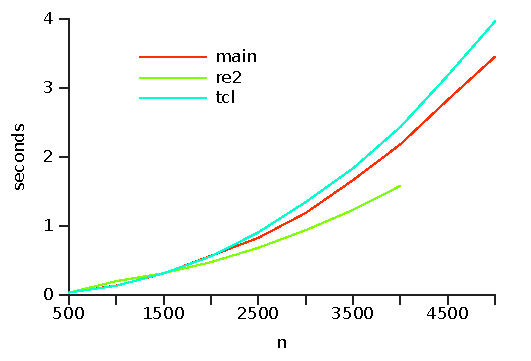
\includegraphics{benchmarks/backtrackingworstcase_maintclre2_normal.pdf}
\caption{A backtracking worst-case: Main, Tcl and RE2 runtimes.}
\label{fig:backtrackingworstcase_maintclre2_normal}
\end{figure}

\begin{figure}
\centering
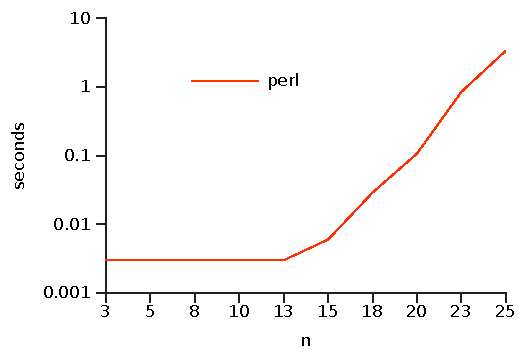
\includegraphics{benchmarks/backtrackingworstcase_perl_log.pdf}
\caption{A backtracking worst-case: Perl runtime on a logarithmic scale.}
\label{fig:backtrackingworstcase_perl_log}
\end{figure}

The runtimes can be seen in figures
\ref{fig:backtrackingworstcase_maintclre2_normal} and
\ref{fig:backtrackingworstcase_perl_log}. As anticipated: Perl
exhibits very poor performance. The slope on figure
\vref{fig:backtrackingworstcase_perl_log} and the logarithmic scale
suggest that Perl runs in time exponential in $n$. This is not
surprising considering that the \textsf{?} matches greedily,
meaning it will first try to consume a character from input. The only
way that the regular expression matches the string is if all the
quantifiers consume no input. There are $2^n$ possible ways for the
quantifiers to consume and not consume a character. The backtracking
engine has to search through all the $2^n$ possible solutions to find
the matching one, since it matches greedily.

In figure \vref{fig:backtrackingworstcase_maintclre2_normal} we do not
see much difference in the performance of Main, RE2 and Tcl. RE2 stops
before the others, it has a upper limit on how much memory it will
consume. The limit is user (compile time) defined for RE2\todo{jan: changed}. This limit could have been set to a value that would allow
RE2 to continue matching with Main and Tcl. We chose not to do this,
because we wanted to demonstrate this feature in RE2. This feature is
especially useful in setups where memory is very tight or you accept
regular expressions from untrusted sources, but can obviously also be considered a
nuisance in other situations where you do not want to fiddle with this
limit, but just want to make RE2 do your matches.

As a side note, we found that if we added a \textsf{b}\todo{jan: does what?} at the end of
the regular expression we would suddenly see marked improvements in
the runtimes of Perl. Using a backtracking algorithm it would still
take time exponential in $n$ to decide they did not match, but Perl
scans the input string for all literals in the regular expressions,
and it quickly discovers that there is no \textsl{b} in the input
string, so therefore the regular expression can not match the
string. 


\subsubsection{Memory usage}

\begin{figure}
\centering
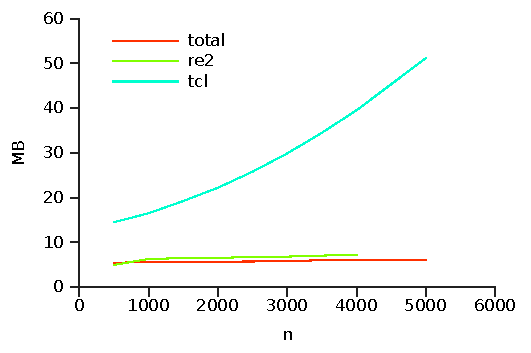
\includegraphics{benchmarks/memory/backtrackingworstcase_mem_totalre2tcl.pdf}
\caption{A backtracking worst-case: Total, Tcl and RE2 memory usage.}
\label{fig:backtrackingworstcase_mem_maintclre2_normal}
\end{figure}

\begin{figure}
\centering
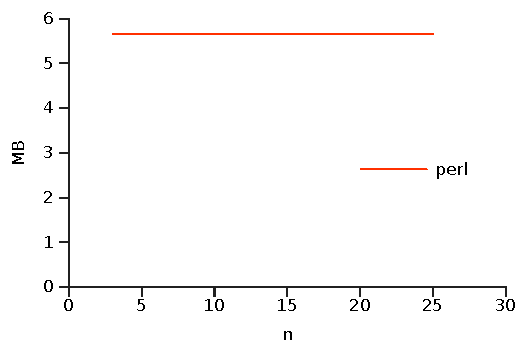
\includegraphics{benchmarks/memory/backtrackingworstcase_mem_perl.pdf}
\caption{A backtracking worst-case: Perl memory usage.}
\label{fig:backtrackingworstcase_mem_perl_log}
\end{figure}

Memory usage is depicted in figures
\ref{fig:backtrackingworstcase_mem_maintclre2_normal} and
\ref{fig:backtrackingworstcase_mem_perl_log}. For our program we have
added up the memory usage of the individual programs and displayed
them under the total header. 

In figure \vref{fig:backtrackingworstcase_mem_maintclre2_normal} we
again note that RE2 stops before the other two because of memory limitations. The memory usage of our programs and RE2 does not appear
to be more than linear in the input size, Tcl looks more like some
quadratic function. It is hard to give a good explanation to this
without knowing Tcls regular expression better, even if it did use a
NFA for this match the size should still be linear in the input. Tcl
has the same asymptotic runtime performance as Main and RE2, but with
bigger constants; all that extra memory spent is not being put to
good use. 

Figure \vref{fig:backtrackingworstcase_mem_perl_log} shows Perls
memory usage. It is hard to say anything useful based on that graph,
the values for $n$ are too small. Unfortunately, due to the exponential run-time\todo{jan: changed from nature} of
the problem it is not viable to increase them.

\subsection{A DFA worst-case}

Using superscripts to denote string repetition, constructing a DFA
from the regular expression \textsf{(a\textbar b)*a(a\textbar b)$^n$}
results in a exponential blow up of the state count. For example will
\textsf{(a\textbar b)*a(a\textbar b)$^3$} translate to
\textsf{(a\textbar b)*a(a\textbar b)(a\textbar b)(a\textbar
  b)}. Acceptance with a DFA is decided in time linear to the size of
the input string, but we would still have to store the DFA which takes
space exponential in the size of the regular expression. We expect any
regular expression engine using DFAs to do poorly on this
benchmark. The engines that can be expected to use DFAs are RE2 and
Tcl, but both can switch method according to need. 


For this experiment we used the programs \texttt{main} and
\texttt{ismatch}. The script used for the backtracking worst case is
in sections \vref{sec:dfaworstcase.pl} and
\vref{sec:dfaworstcase_mem.pl}.


\subsubsection{Runtimes}

\begin{figure}
\centering
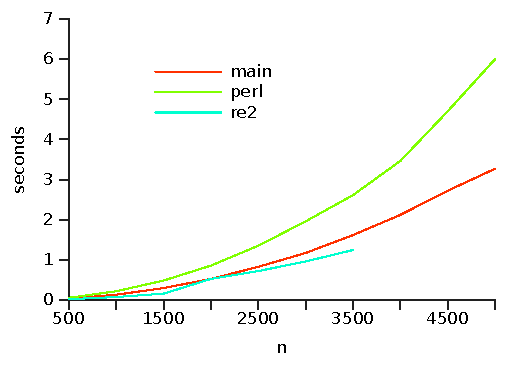
\includegraphics{benchmarks/dfaworstcase_mainre2perl_normal.pdf}
\caption{A DFA worst-case: Main, RE2 and Perl runtimes.}
\label{fig:dfaworstcase_mainre2perl_normal}
\end{figure}

\begin{figure}
\centering
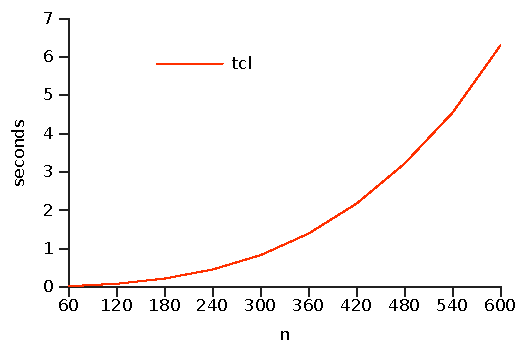
\includegraphics{benchmarks/dfaworstcase_tcl_normal.pdf}
\caption{A DFA worst-case: Tcl runtimes.}
\label{fig:dfaworstcase_tcl_normal}
\end{figure}

In figures \ref{fig:dfaworstcase_mainre2perl_normal} and
\ref{fig:dfaworstcase_tcl_normal} we have the figures displaying the
runtimes of the various programs. Again we note that RE2 stops before
the others, see above. Tcl stands out with significantly lower
performance, but none appears to have exponential or worse asymptotic
behavior. This would suggest that Tcl chooses to use a DFA in some
form for this match and RE2 falls back on something else.


\subsubsection{Memory usage}

\begin{figure}
\centering
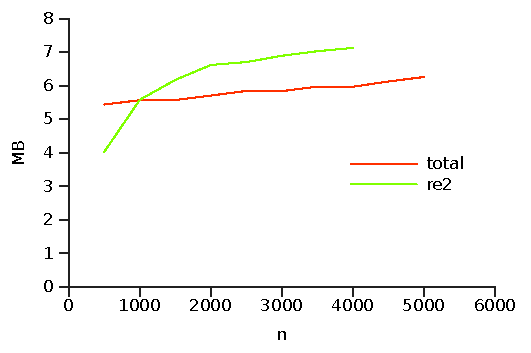
\includegraphics{benchmarks/memory/dfaworstcase_mainre2.pdf}
\caption{A DFA worst-case: Main and RE2 memory usage.}
\label{fig:dfaworstcase_mem_mainre2}
\end{figure}

\begin{figure}
\centering
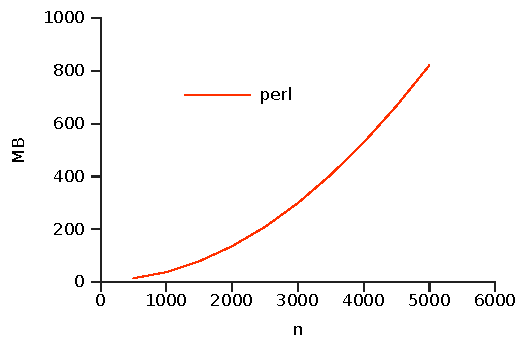
\includegraphics{benchmarks/memory/dfaworstcase_perl.pdf}
\caption{A DFA worst-case: Perl memory usage.}
\label{fig:dfaworstcase_mem_perl}
\end{figure}

\begin{figure}
\centering
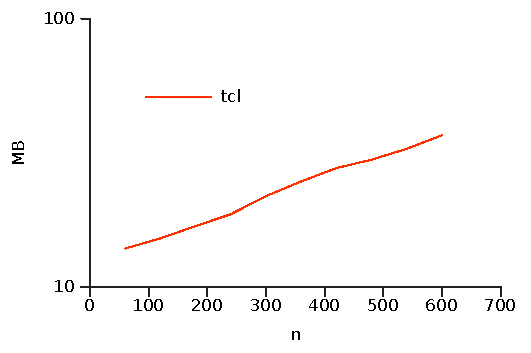
\includegraphics{benchmarks/memory/dfaworstcase_tcl_log.pdf}
\caption{A DFA worst-case: Tcl memory usage.}
\label{fig:dfaworstcase_mem_tcl_log}
\end{figure}

The memory usage proved to be a more complicated matter than the
runtimes, see figures \ref{fig:dfaworstcase_mem_mainre2},
\ref{fig:dfaworstcase_mem_perl} and \ref{fig:dfaworstcase_mem_tcl_log}
display.

Our programs and RE2 appears to be using memory linear in the size of
the regular expression. There is a sharp rise in memory consumed by
RE2 for $n$ smaller than about 1000. This would indicate that RE2 uses
a DFA until the exponential factor becomes to big and forces it to
switch method. 

Perls memory usage is mapped in figure
\vref{fig:dfaworstcase_mem_perl}. Compared to our programs Perl uses
rather a lot of memory. It seems to be increasing in a quadratic
manner.\todo{investigate further}

In figure \vref{fig:dfaworstcase_mem_tcl_log} we have Tcls memory
usage mapped. Note the logarithmic scale. Our suspicion that Tcl uses
a DFA is confirmed by the memory usage, which appears to be
exponential in the size of the regular expression. 


\subsection{Extracting an email-address}

This is the first of our real world benchmarks. We will be extracting
an email-address from a string of text. Since we can not do partial
matches, we will be constructing strings of increasingly long
email-addresses. The regular expression is taken from
\cite{veanes}. Unlike the two previous benchmarks, the regular
expression is kept constant and does not grow.

Since we are extracting a value we are using \texttt{main},
\texttt{groupings\_all}, \texttt{trace} and \texttt{serialize} for
this match. The scripts can be found in sections \vref{sec:email.pl},
\vref{sec:email_mem.pl} and \vref{sec:email_mbvsize.pl}

\subsubsection{Runtimes}

\begin{figure}
\centering
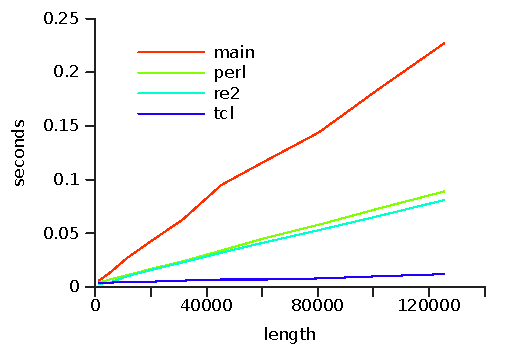
\includegraphics{benchmarks/email.pdf}
\caption{Extracting an email-address: Runtimes.}
\label{fig:email}
\end{figure}

In figure \vref{fig:email} contains the runtimes. All appear to be
running in time linear to the input string, with Tcl clearly having
the lowest constants and our programs the largest. 


\subsubsection{Memory usage}
\begin{figure}
\centering
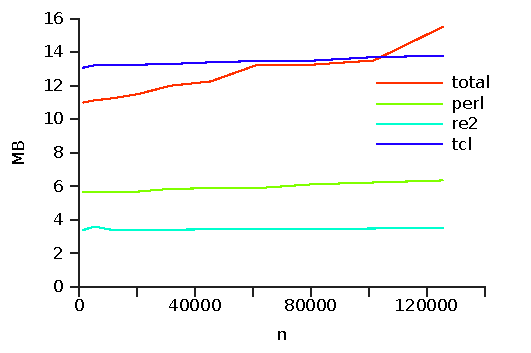
\includegraphics{benchmarks/memory/email_mem.pdf}
\caption{Extracting an email-address: Memory usage.}
\label{fig:email_mem}
\end{figure}

\begin{figure}
\centering
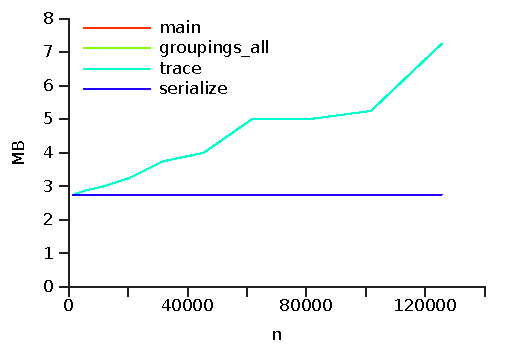
\includegraphics{benchmarks/memory/email_mem_individual.pdf}
\caption{Extracting an email-address: Individual programs memory usage.}
\label{fig:email_individual_mem}
\end{figure}

\begin{figure}
\centering
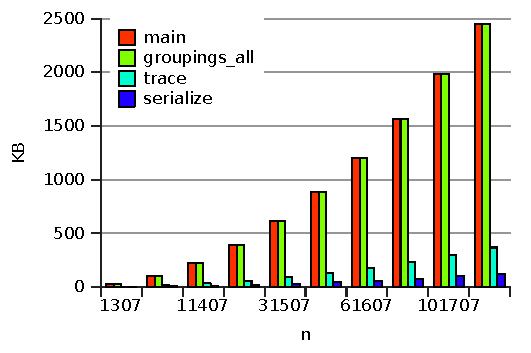
\includegraphics{benchmarks/memory/email_mbvsize.pdf}
\caption{Extracting an email-address: Sizes of output from individual
  programs.}
\label{fig:email_mbvsize}
\end{figure}


\begin{figure}
\centering
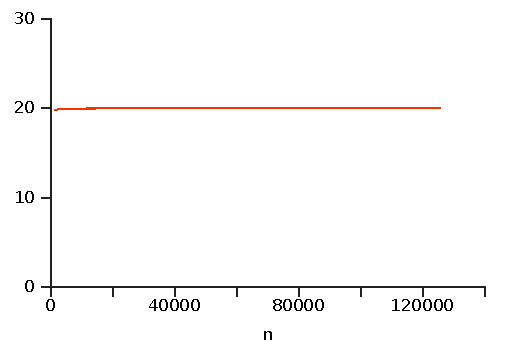
\includegraphics{benchmarks/memory/email_mbvsize_relative.pdf}
\caption{Extracting an email-address: The relationship between input
  size to \texttt{trace} and size of input string.}
\label{fig:email_mbvsize_relative}
\end{figure}


In figure \vref{fig:email_mem} we have the memory usage of the
programs. All programs except ours seem to be using memory linear in
the input string. We seem to be using memory in a stepped manner. This
correlates well with our scheme for memory management in
\texttt{trace}: We double the amount of memory used every time we run
out. This is confirmed by figure \vref{fig:email_individual_mem},
which displays the memory usage for the individual programs. Here we
see that all our programs except \texttt{trace} use a constant amount
of memory. It is hard to tell from figures
\ref{fig:email_individual_mem} and \vref{fig:email_mem} if the memory
used is linear in the input string. What we need to know is the size
of the mixed bit-values compared to the input string; we have
displayed this in figure \vref{fig:email_mbvsize} where we have the sizes
of the output from the individual programs. We did not put in a
separate column for the size of the input string since this is
exactly the same as the size of the output from
\texttt{serialize}. There is a linear relationship between the output
of \texttt{groupings\_all} and \texttt{serialize}: The first is 20
times bigger than the latter. See figure
\vref{fig:email_mbvsize_relative}.

\subsection{Extracting a number}

Our fourth and last benchmark is also a real world example taken from
\cite{veanes}. This one extracts a number from a string. We can not do
partial matches, so again we will be using a string consisting of
increasingly large numbers. The regular expression is constant.

We will be extracting a number, so we will be using programs
\texttt{main}, \texttt{groupings\_all}, \texttt{trace} and
\texttt{serialize} for this match. The scripts can be found in
sections \vref{sec:number.pl}, \vref{sec:number_mem.pl} and
\vref{sec:number_mbvsize.pl}.


\subsubsection{Runtimes}

\begin{figure}
\centering
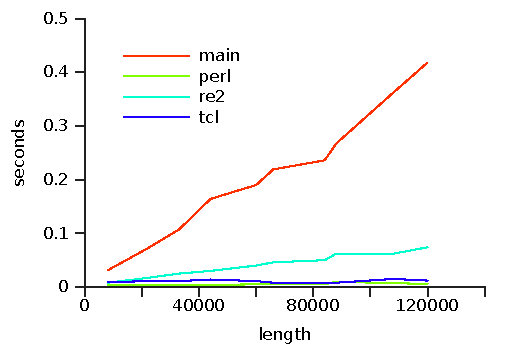
\includegraphics{benchmarks/number.pdf}
\caption{Extracting a number: Runtimes.}
\label{fig:number}
\end{figure}

In figure \vref{fig:number} we have the runtimes for this
benchmark. They all appear to be linear in the size of the input
string. Our programs clearly have bigger constants than the rest. 


\subsubsection{Memory usage}


\begin{figure}
\centering
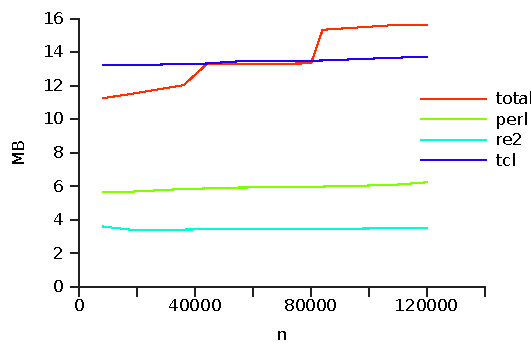
\includegraphics{benchmarks/memory/number_all.pdf}
\caption{Extracting a number: Memory usage.}
\label{fig:number_mem}
\end{figure}


\begin{figure}
\centering
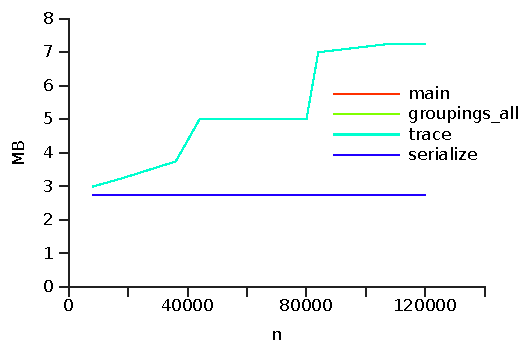
\includegraphics{benchmarks/memory/number_individual.pdf}
\caption{Extracting a number: Individual programs memory usage.}
\label{fig:number_mem_individual}
\end{figure}

\begin{figure}
\centering
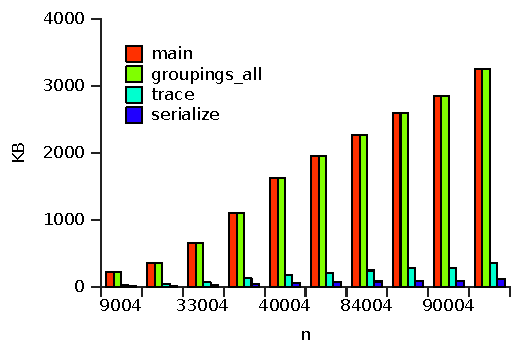
\includegraphics{benchmarks/memory/number_mbvsize.pdf}
\caption{Extracting a number: Sizes of output from individual programs.}
\label{fig:number_mem_mbvsize}
\end{figure}


\begin{figure}
\centering
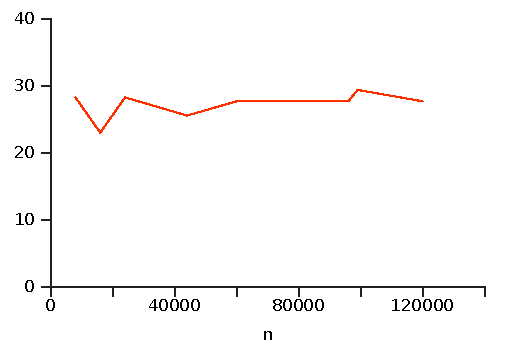
\includegraphics{benchmarks/memory/number_mbvsize_relative.pdf}
\caption{Extracting a number: The relationship between input size to
  \texttt{trace} and size of input string.}
\label{fig:number_mem_mbvsize_relative}
\end{figure}


In figure \vref{fig:number_mem} we have the memory usage. We clearly see the same pattern as in the extracting an
email address benchmark: that our programs use memory in a stepped but linear
manner and the rest use memory linear in the size of the input
string. We investigate further, see figure
\vref{fig:number_mem_individual} for the individual programs memory
usage. All our programs, except \texttt{trace} use a constant amount
of memory. The steps in the memory usage of \texttt{trace} is even
more pronounced in this figure. See above note on memory management
strategy in \texttt{trace} for explanation. The relationship between
the sizes of the output from the different programs is displayed in
figure \vref{fig:number_mem_mbvsize}. The size of the input string is
exactly the same as the output from \texttt{serialize}. For greater
clarity we have the relationship between the input size to
\texttt{trace} and the size of the input string displayed in figure
\vref{fig:number_mem_mbvsize_relative}. We do not observe the same
fixed relationship between the two as we did in the extracting an
email address benchmark - there seem to be no increasing trend. We
generate between 20 and 30 mixed bit-values per byte in the input
string.


\subsection{Large files}

We also did some experiments involving a large (333.5MB) log file. The
log file was lifted from another project where it was used to gather
data on file access \cite{jan2010}. The data in the log file was
aggregated, one line at a time, using some regular expressions that
could easily be translated for use in our regular expression
engine. Our experiment consisted of replicating the aggregation of
data. This is where our problems with this experiment began: We tried
to read the whole file at the same time, since the current version of our framework has no support for line-by-line reads. 
After some time this resulted in an out of memory error. 

This is not a problem specific for our framework; we observe that this operation on some
other existing implementation, such as Perl, also results in an out of
memory error. 

The lesson in this experiment is that we lack some way of applying
regular expression one line at a time. We could have tried applying
the regular expressions with the help of \texttt{awk}, but it seemed
superfluous invoking our pipeline of programs when \texttt{awk}
already has a perfectly good regular expression engine built in. Our
other choice would have been making a shell-script and used a loop and
\texttt{cat}. 


\subsection{Conclusion}

We observe that our programs do not suffer from either the
backtracking worst-case or the DFA worst-case problems.

\paragraph{Simple acceptance} We can compete on even footing with the
best when it comes to a simple acceptance decision. Our main program
combined with the 'match' filter is fast and uses memory linear in the
size of the regular expression.

\paragraph{Capturing groups} When it comes to the more complicated
task of capturing the contents of groups, we are lagging behind. The
task of capturing groups is achieved by a 4 programs long pipe in our
framework. Even if all of them only used memory linear in the length
of the regular expression, the overhead of running separate programs
add up.  The 'trace' filter uses memory linear in the size of the
input string. While this is obviously not quite as good as the other
filters, it is nevertheless a good result, we have managed to separate
this functionality into an independent component.

An obvious drawback is the constant basic overhead of having four
individual programs instead of one. We note however that this is
currently completely unoptimized and that this cost will not rise
relative to either input. It is also still quite low; it would likely only be a relevant problem in a demanding environment
such as embedded devices.

The other main problem is the blow up of the size of the mixed
bit-values. We have previously discussed potential solutions to this
problem.
